

% \paragraph{Data Imbalance Problems.}
% In the real world, dogs and cats outnumber rare animals, and this characteristic of nature is reflected in the curation of data.
% These data imbalance problems can cause poor generalization and many issues in finance, healthcare, and autonomous driving.
% In this paper, we tackle long-tailed recognition, fairness, and model robustness to spurious correlation, which are related closly from the data imbalacne perspective.

% Imbalance in data
Data imbalance can lead to
% cause poor
suboptimal generalization and many challenges
% issues
in practical application scenarios, \eg, finance, healthcare, and autonomous driving.
The data imbalance problem is a common source of different imbalance sub-problems: long-tailed recognition, model fairness, and model robustness to spurious correlation.
% This work is related to the data imbalance problem, and 
We brief the related work on the associated sub-problems and on using synthetic data for machine learning tasks.
% review its associated sub-problems and using synthetic data.
% : class imbalance (long-tail), fairness, and spurious correlation.
% In this paper, we tackle which are related closly from the data imbalacne perspective.



% \begin{wrapfigure}{r}{0.45\linewidth}
%     \centering
%     \vspace{-6mm}
%     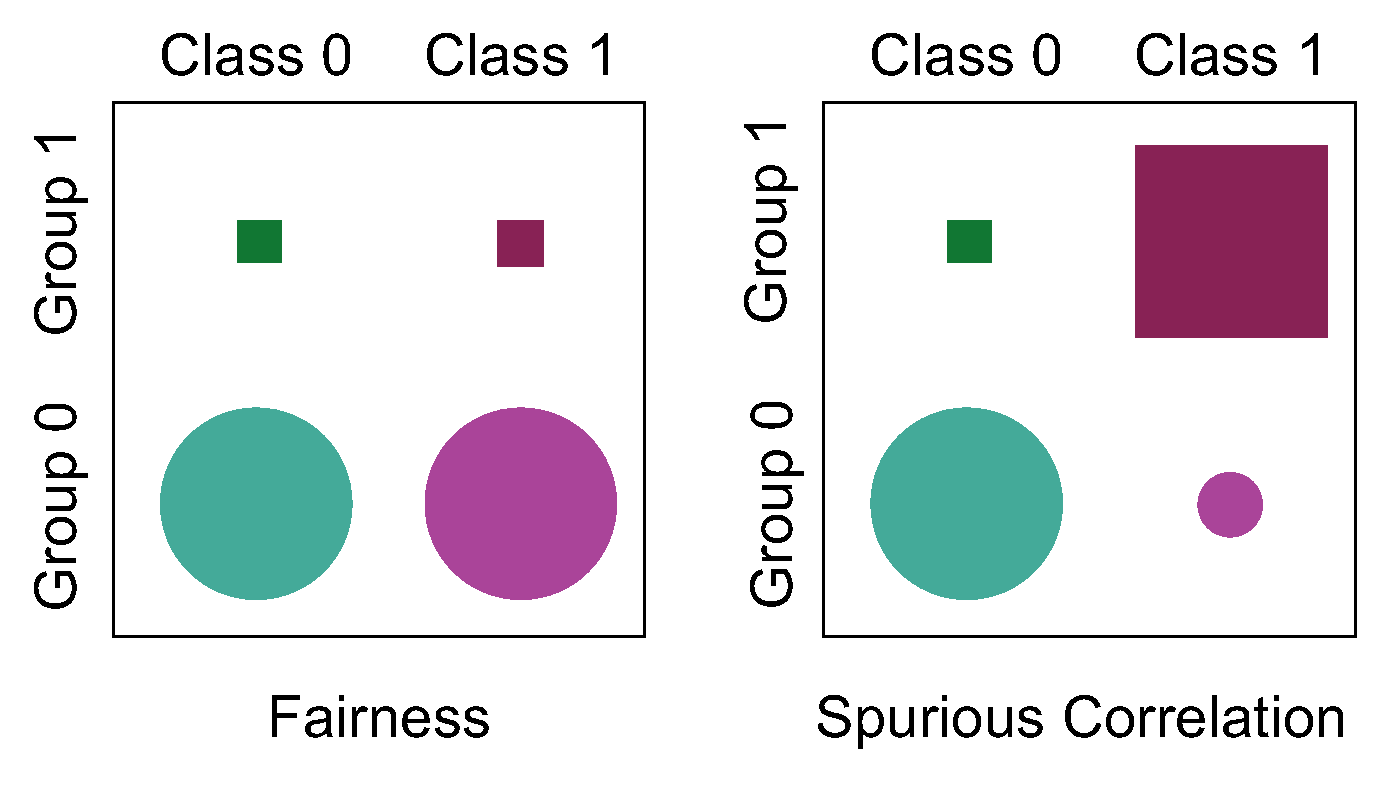
\includegraphics[width=1.0\linewidth]{figures/group_imbalance_teaser.pdf}
%     \caption{\textbf{Overview of fairness and spurious correlation from the data perspective.}
%     The size of a shape represents the amount of data. The same shape stands for the same group, and the same color for the same class.\vspace{-3mm}}
%     % 
%     \label{fig:group_imbalance_teatures}
% \end{wrapfigure}

% It is well-known that long-tailed recognition~\cite{cui2019class,zhang2023deep}, where their training data follow Pareto distribution, is one of the class imbalance problems.
% Long-tailed distribution, \ie, Pareto distribution, is natural in the real world, which has a class imbalance.
% Dogs and cats outnumber rare animals, and this characteristic of nature is reflected in the curation of data.


% (see \Fref{fig:group_imbalance_teatures}).

% Model robustness is related to spurious correlations that some classes appear with certain patterns, \ie, spurious or shortcut features~\cite{geirhos2020shortcut, scimeca2022iclr, kirichenko2023last}.

% for deep neural networks 

% Since the long-tail distribution, model robustness, and model fairness are related closely from the data imbalance perspective, we handle these three data imbalance problems.



\paragraph{Long-tailed recognition.}
Long-tailed distribution is inherent to the real world~\cite{cui2019class,zhang2023deep}.
There are two main streams in the realm of re-balancing classes, including re-sampling~\cite{shen2016relay,park2022majority,kim2020m2m,liu2019large} and re-weighting~\cite{he2009learning,samuel2021distributional, cao2019learning, ren2020balanced, lin2017focal, ryou2019anchor, cui2019class}.
The re-weighting methods share a similar mechanism to weighting minority classes inverse-proportionally to the number of instances. 
% less frequent class by the inverse of frequency~\cite{he2009learning, cui2019class}.
The re-sampling methods weight the samples in minority classes by more frequently sampling with replacement so that the training model can see the uniform number of samples across classes.

There are other approaches 
% to tackle the problem
by designing loss functions.
Ryou~\etal\cite{ryou2019anchor} and Lin~\etal\cite{lin2017focal} 
% design loss functions that 
induce adaptive re-weighting effects during training.
The others take into account margin~\cite{cao2019learning} or balance of softmax~\cite{ren2020balanced} in the loss design.
% Also, there are other approaches to take into account other factors in the loss design: margin~\cite{cao2019learning} or balance of softmax~\cite{ren2020balanced}.
Wang~\etal\cite{wang2021longtailed} take a completely different approach; model selection given diversely pre-trained classifiers.
In addition, Ye-Bin~\etal\cite{yebin2023textmania} propose
% proposes
TextManiA, visual feature augmentation for sparse samples, which shows improved performance in long-tailed distribution.


\paragraph{Model fairness.} 
In fairness~\cite{narayanan2018translation, hardt2016equality, 10.1145/2783258.2783311}, researchers have tackled the issue of model bias, where accuracy varies based on 
% the unfairness that the model accuracy is different depending on
sensitive attributes such as race, age, and ethnicity.
Model fairness is also related to data imbalance because the number of samples of some sensitive groups is lower than that of the major groups.
Fairness has predominantly been tackled using loss weighting and batch sampling.
A loss weighting algorithm~\cite{jung2023reweighting} proposes fairness optimization, where they minimize the worst-case loss of the group by adaptively weighting losses.
% during training.
Batch sampling approaches~\cite{kamiran2012data, roh2020fairbatch} take an adaptive sampling strategy by considering sensitive information rather than uniform sampling.
Zeng~\etal\cite{zeng2022fair} take a post-calibration approach after training
% with the above existing method
to calibrate the classifiers.


% arjovsky2019invariant,bahng2020learning,sagawa2019distributionally,teney2020unshuffling,tartaglione2021end, lee2021learning,LfF,liu2021just, kim2022learning,yao2022improving,hwang2022selecmix,kirichenko2023last,cao2019learning,ren2020balanced,samuel2021distributional, shen2016relay,park2022majority,kim2020m2m,liu2019large
\paragraph{Spurious correlation.}
% While the spurious correlation problem shares similarities with fairness, it 
The spurious correlation problem is related to the robustness of models against misleading correlations.
DNNs are susceptible to falling into shortcuts that capture the most frequently observed patterns in a class regardless of true causality;
it is called spurious correlation or shortcut problems~\cite{geirhos2020shortcut, scimeca2022iclr, kirichenko2023last}.
It is never desirable to rely on spurious features that degrade the generalizability of DNNs~\cite{sagawa2019distributionally, liu2015deep}.
The spurious correlation problem is also dealt with similar approaches to the above two tasks: weighting~\cite{sagawa2019distributionally,LfF,kim2022learning}, sampling~\cite{idrissi2022simple, sagawa2020investigation}, augmentation~\cite{lee2021learning,yao2022improving,hwang2022selecmix}, and post-calibration~\cite{liu2021just, kirichenko2023last, lee2022surgical}.


\paragraph{Summary of data imbalance problems.}
While researchers have developed algorithms for each task separately, three different tasks sourced from data imbalance have mainly been tackled in the shared perspective, \ie, 
% re-balancing; 
up-weight loss values or sampling probabilities of minor groups using group or sensitive information.
However, they have focused only on algorithmic parts by limiting their methods to exploit the given imbalance dataset, where the inherent imbalance still remains.

In this work, we shed light on the overlooked convention to go beyond the given bounded dataset.
We exploit the synthetic data from the generative foundation models~\cite{rombach2022high, saharia2022photorealistic, nichol2021glide} to take flexibility and controllability so that we can populate the long-tailed training data distribution to become a uniform distribution, which mitigates the imbalance problem itself.
We observe that this simple correction of class distribution with synthetic data can significantly improve the worst-case accuracy and fairness of DNNs.
To our best knowledge, our work is the first work that demonstrates improved or competitive performance with generated synthetic data for both class imbalance and fairness tasks.

\paragraph{Using synthetic data in machine learning tasks.}
To overcome the lack of data or sensitive issues of data, \eg, licensing and privacy concerns, recent approaches have started to leverage synthetic data for their tasks of interest:
classification~\cite{antoniou2017data, tran2017bayesian}, segmentation~\cite{sandfort2019data, zhang2021datasetgan}, re-identification~\cite{zheng2017unlabeled}, motion estimation~\cite{dosovitskiy2015flownet, mayer2016large, sun2021autoflow, han2022realflow, oh2018learning}, computational photography~\cite{pan2021dual}, and representation learning~\cite{jahanian2021generative}.
Recently, deep generative models~\cite{rombach2022high, saharia2022photorealistic, nichol2021glide} have shown promising results in generating realistic and high-quality samples, stemming from the goal of modeling the real data distribution.
In particular, the image generation conditioned on text provides great controllability and flexibility, which has the potential to be used for a variety of tasks, such as 3D reconstruction~\cite{poole2023dreamfusion, raj2023dreambooth3d, chen2023fantasia3d} and image recognition~\cite{trabucco2023effective, he2022synthetic, azizi2023synthetic}.
In this work, we explore the use of a pre-trained foundation diffusion model to mitigate data imbalance problems.



